%% Lee
%% In dissertation, change 
%    section* to chapter 
%    subsection* to section
%    subsubsection* to subsection


% #######################################################################################################################################
\chapter{Detailed System Description}
\label{sec:Detailed System Description}

A detailed flow diagram and block diagram of the sub-system column can be seen in figures \ref{fig:DetailedFlowDiagram} and \ref{fig:DetailedBlockDiagram} respectively.
\begin{figure}[h]
% the [] contains position info e.g. [!t] means here
\centering
\captionsetup{justification=centering}
\captionsetup{width=.9\linewidth}
\centerline{
\mbox{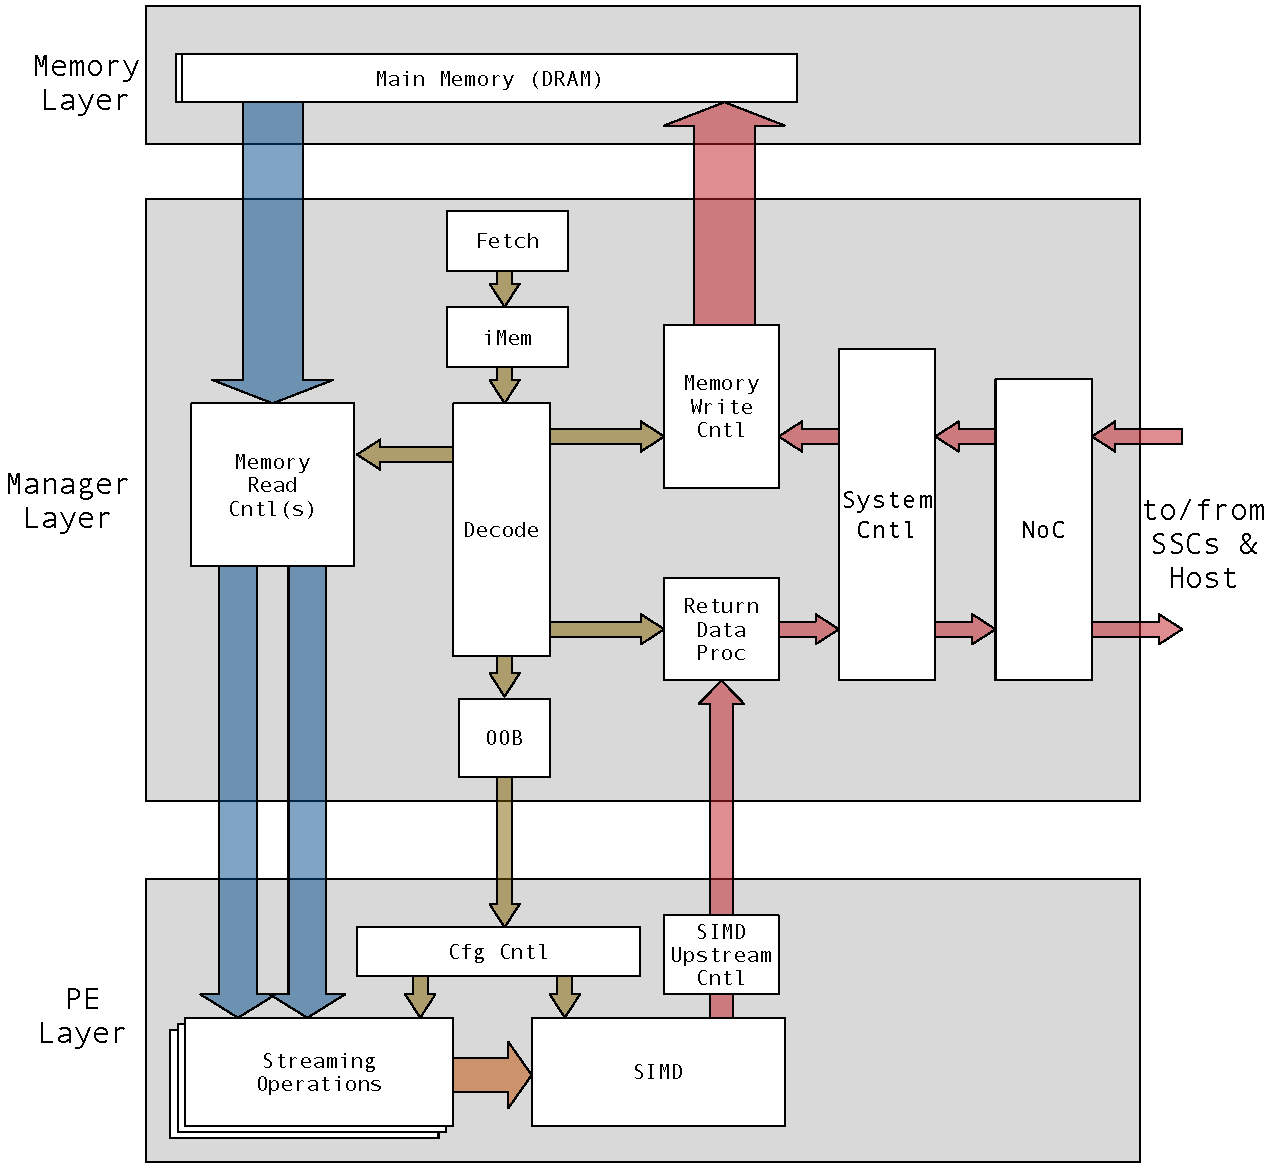
\includegraphics[scale=0.07]{DetailedFlowDiagram}}
}
\center\caption{Sub-System Column (SSC) Flow Diagram}
\label{fig:DetailedFlowDiagram}
\end{figure}

\begin{sidewaysfigure}[h]
% the [] contains position info e.g. [!H] means here
% H 	Place exactly at spot in source text
% h 	Place approximately at spot in source test
% t 	Place at top of page
% b 	Place at bottom of page
% p 	Place on page for floats only
% ! 	Override internal LaTeX parameters for determining float position
\centering
\captionsetup{justification=centering}
\captionsetup{width=0.9\textwidth}
\centerline{
\mbox{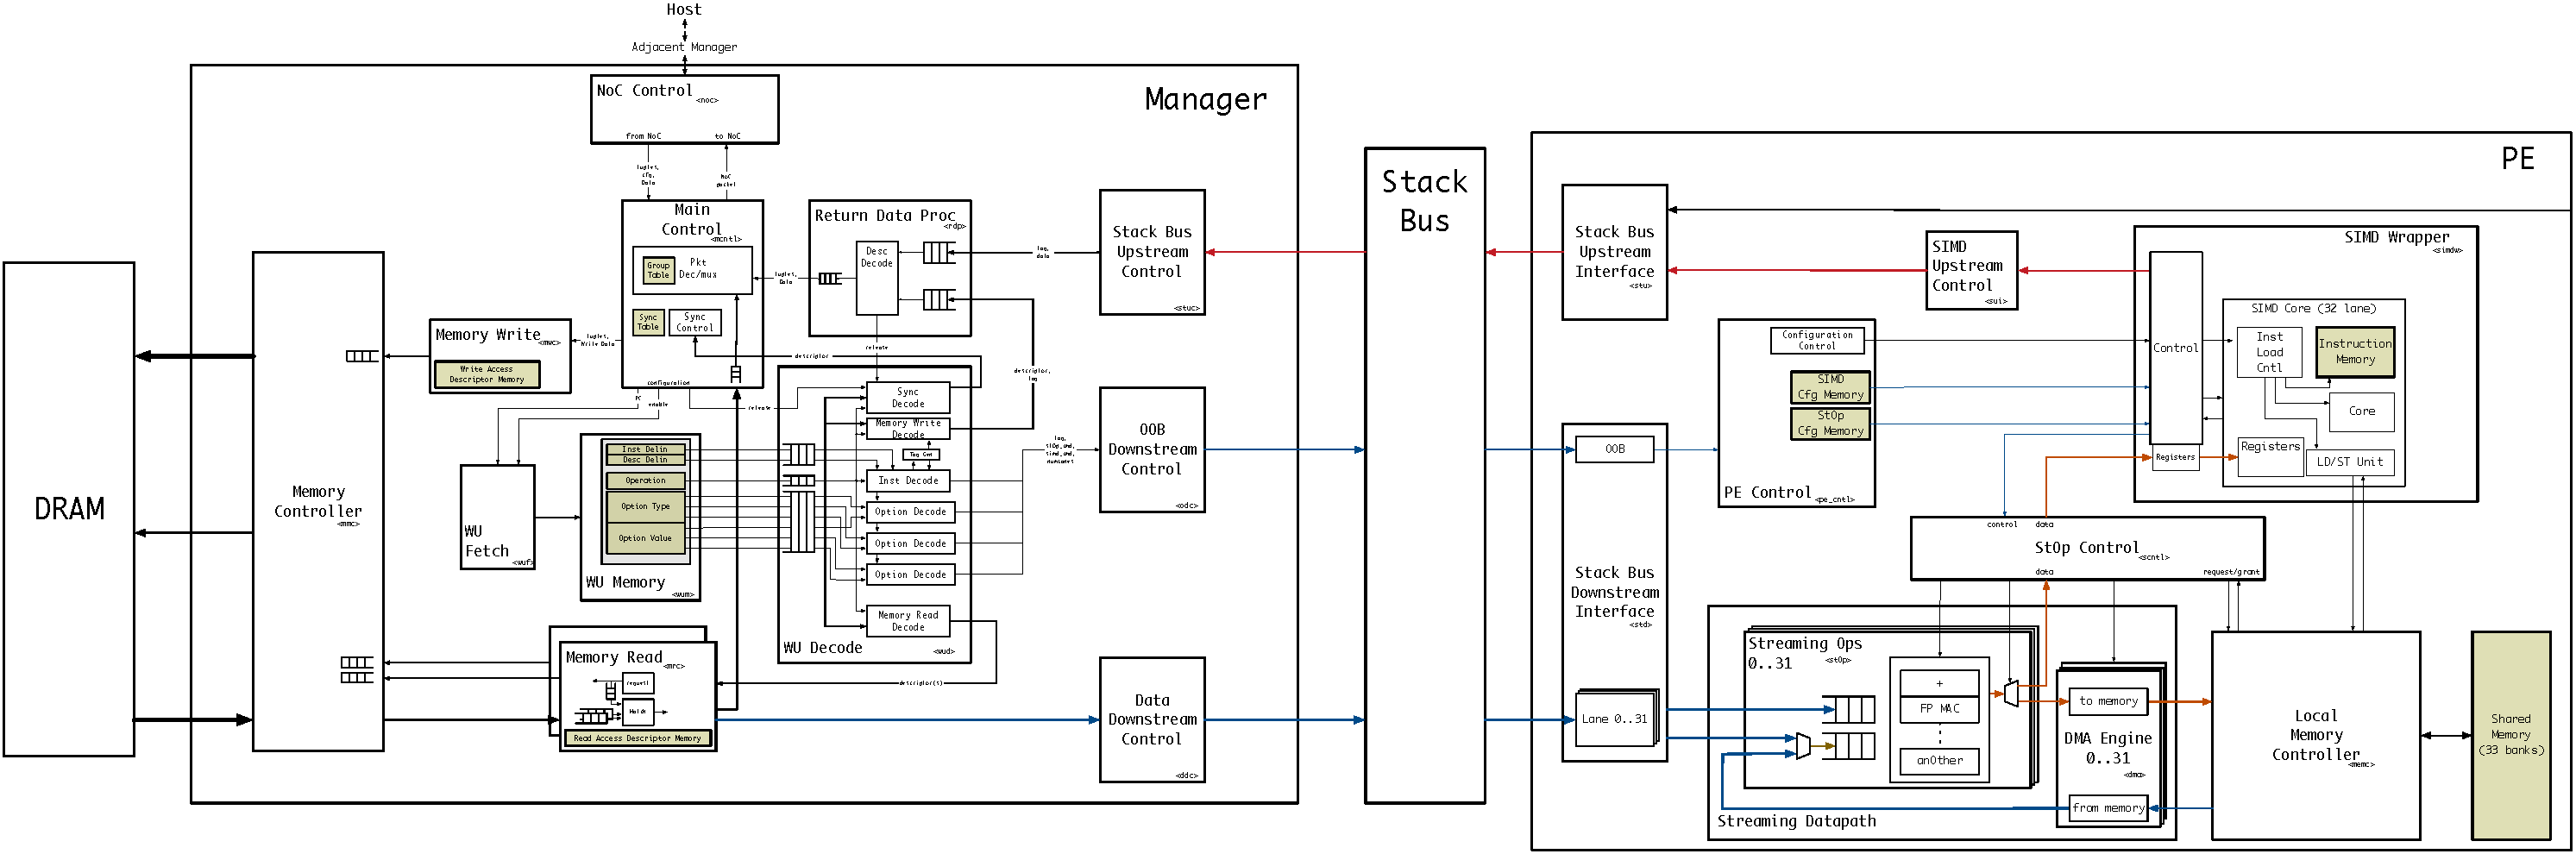
\includegraphics[angle=0, width=1.0\textwidth]{DetailedBlockDiagram}}
}
\center\caption{Sub-System Column (SSC) Block Diagram}
\label{fig:DetailedBlockDiagram}
\end{sidewaysfigure}

\section{Manager}
\label{sec:manager}

A block diagram of the manager can be seen in figure \ref{fig:Manager block diagram}.
\begin{figure}[h]
\centering
\captionsetup{justification=centering}
\captionsetup{width=.9\linewidth}
\centerline{
\mbox{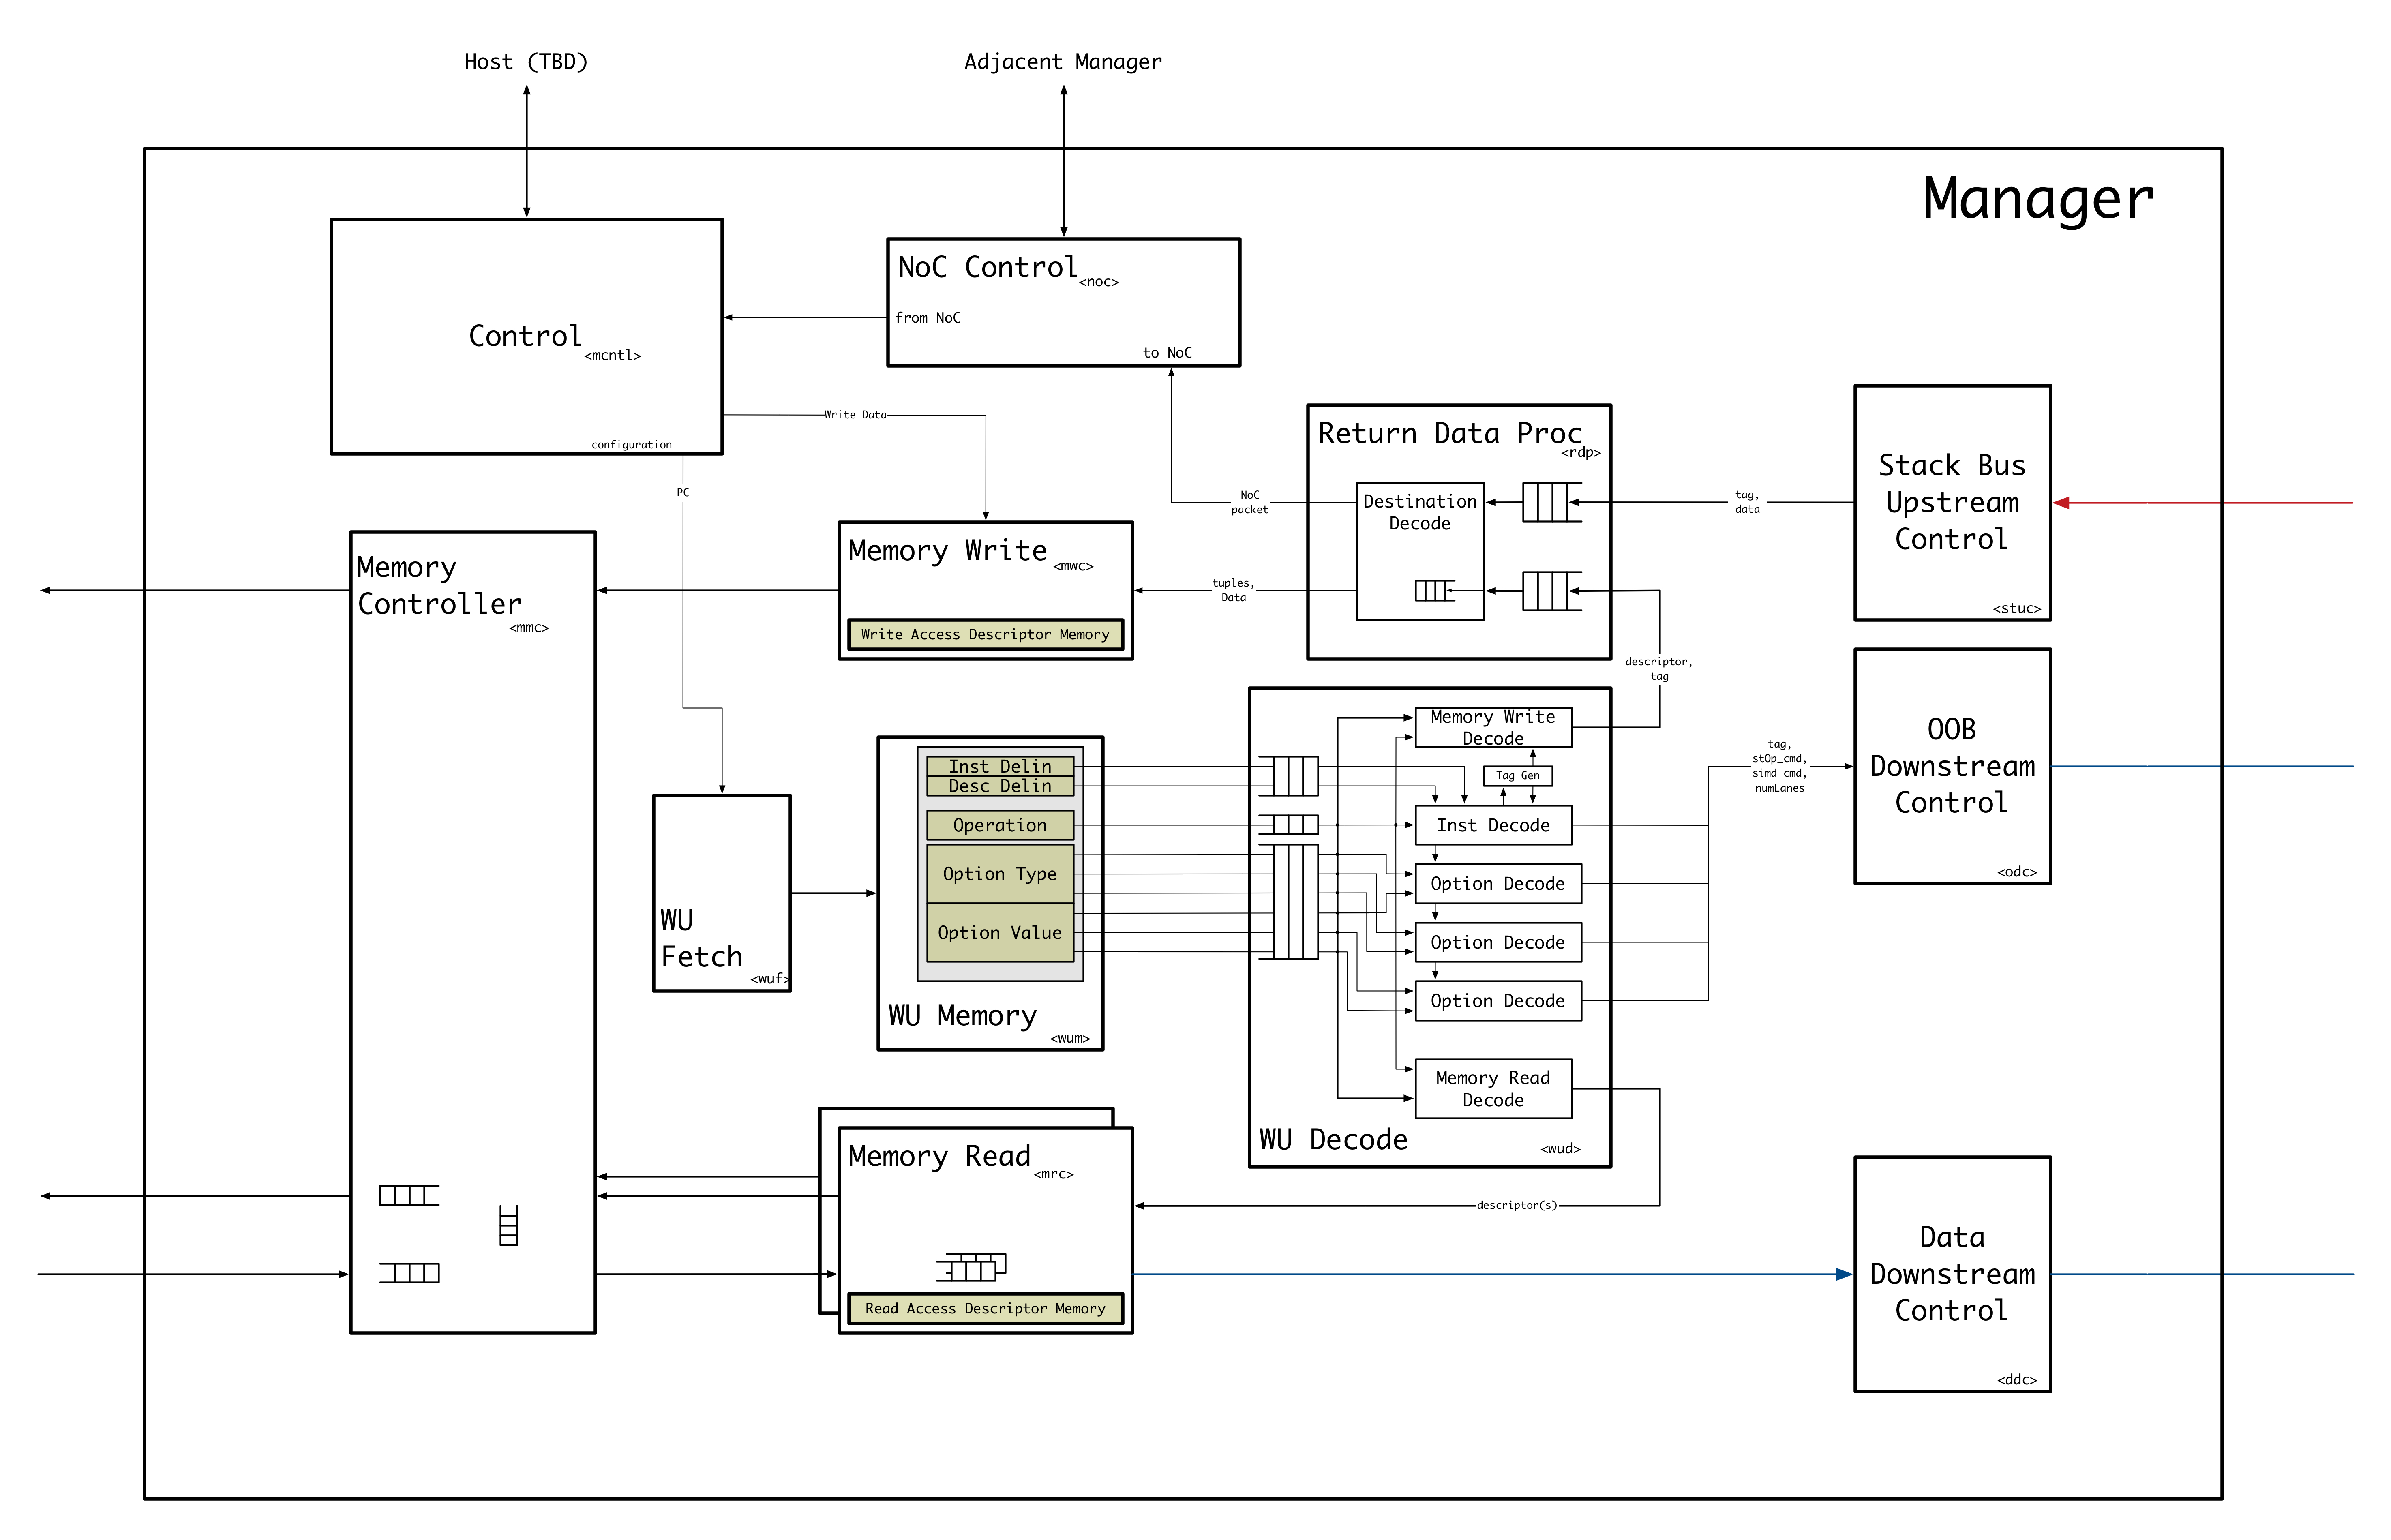
\includegraphics[width=1\linewidth]{Manager}}
}
\center\caption{Manager block diagram}
\label{fig:Manager block diagram}
\end{figure}

\subsection{Instruction Decoder}
\label{sec:Instruction Decoder}

\subsubsection{Operation Decode}
\label{ssec:operationDecode}

In figure \ref{fig:Manager block diagram}, instructions are read from WU memory by the WU fetch block and the output of the memory is passed to the WU decoder block.

\subsubsection{Decoding Compute Instructions}
\label{sec:Decoding Compute Instructions}

The operation descriptor is decoded and a \ac{stop} pointer and a \ac{simd} \ac{pc} pointer are extracted. 
A sequential tag is generated and along with the \ac{stop} and \ac{simd} pointers and immediately sent to the \ac{pe} inside an \ac{oob} control packet.
The \ac{stop} pointer specifies what streaming operation is to take place on the data directly streamed to the \ac{pe}. 
The SIMD pointer is essentially a \ac{pc} counter that the \ac{simd} will jump to to process the result from the \ac{stop}.
The \ac{pe} will immediately start preparing for downstream oeprand data.
If the \ac{simd} operation ncludes result data being returned to the manager, the tag will be included in the upstream result data packet.

The memory read descriptors are decoded to identify the target memory read controller and the storage descriptor pointer directed to the appropriate memory read block.
There is a memory read block associated with each of the operand streams and are responsible for generating memory requests and directing the \ac{dram} data to all the execution lane streams.
A request block inside the memory read block immediately start pre-fetching the memory data by sending memory requests to the \ac{dram}.
A stream block inside the memory read block immediately starts waiting for data from the \ac{dram} and will direct \ac{dram} data to the appropriate execution lane.

The memory write descriptor is decoded and the storage descriptor pointer extracted and along with the tag are sent to the return data processor. The tag is sent to match with the returned data.
Currently the system only allows in-order data but the tag is provided for extensibility.

At this point all the blocks that take part in a compute operation on a group of \acp{an} are perforiming the various tasks.
As mentioned in section \ref{sec:Common Bus Signalling}, the inputs to many blocks employ \acp{fifo}. 
This allows blocks to pipeline tasks to absorb any latencies, they also allow blocks to start sending data to a destination block before that block has been configured to receive the data.
The \ac{fifo} will assert a flow control signal until the block is ready to receive.
In practice, the instruction decode logic batch decodes up to eight instructions and sends descriptor contents to dependent blocks where they are also pipelined.

\subsubsection{Decoding Configuration Instructions}
\label{sec:Decoding Configuration Instructions}

Currently the sync instruction has been implemented.
It is assumed at this point that adequate infrastructure and extensibility has been built into the system to allow implementation without adding significant amouts of logic.

The configuration descriptor contains a single configuration sync option tuple. The 24-bit option value contains a 3-bit mode register identifier and a 21-bit register.
There are currently four mode registers defined, "Send", "Wait", "Pause" and "Flush". Each register has fields specific to the mode (see figure \ref{fig:Sync instruction}).

\paragraph{Sync Send}

The register fields can be seen in register \ref{reg:Sync Send mode register}.
The decoder sends the sync option tuple to the main controller.
A sync \ac{noc} packet is constructed based on the register contents sent over the \ac{noc}.
If the group pointer enable bit is set, the main controller uses the pointer to index into a 64 table. 
Each table entry is a 64-bit bitfield indicating which \acp{ssc} are a part of the group.
If the all flag is set, the sync packet will be sent to all \acp{ssc}.
if the host flag is also set, the host bit in the \ac{noc} packet will be set.
\begin{register}{H}{Sync Send mode register}{}%{0x250} name=example
  \label{reg:Sync Send mode register}
  % sizes 
  %\tiny 	
  %\scriptsize 	
  %\footnotesize
  %\small 	
  %\normalsize 	
  %\large 	
  %\Large 	
  %\LARGE 	
  \vspace{-20pt}
  \regfield{{\scriptsize Mode Reg ID         }}{ 3}{21}{000}%
  \regfield{{\scriptsize Not used            }}{12}{ 9}{{NA}}%
  \regfield{{\scriptsize Group Pointer enable}}{ 1}{ 8}{{en}}%
  \regfield{{\scriptsize Sync Group pointer  }}{ 6}{ 2}{{gPtr}}%
  \regfield{{\scriptsize Send to all SSCs    }}{ 1}{ 1}{{{\tiny all}}}%
  \regfield{{\scriptsize Send to host        }}{ 1}{ 0}{{{\tiny  host}}}%
  %\center\caption{Sub-System Column (SSC) Block Diagram}
  %\reglabel{Reset}\regnewline%
\end{register}

\paragraph{Sync Wait}

The register fields can be seen in register \ref{reg:Sync Send mode register}.
The decoder sends the sync option tuple to the main controller.
The instruction decoder will stop processing any more instructions until the release signal is asserted from the main controller.
The wait option informs the main controller to start expecting sync send packets from other \acp{ssc} and/or the host.
Based on the register values, the main controller will assert the release signal to the instruction decoder only once sync send packets have been received from all specified sources.
If the group pointer enable bit is set, the main controller uses the pointer to index into a 64 table. 
Each table entry is a 64-bit bitfield indicating from which \acp{ssc} a sync send packet should be received.
If the all flag is set, all sync send packets are expected from all \acp{ssc}.
if the host flag is also set, a sync send packet is expected from the host.
\begin{register}{H}{Sync Wait mode register}{}%{0x250} name=example
  \label{reg:Sync Wait mode register}
  \vspace{-20pt}
  \regfield{{\scriptsize Mode Reg ID         }}{ 3}{21}{001}%
  \regfield{{\scriptsize Not used            }}{12}{ 9}{{NA}}%
  \regfield{{\scriptsize Group Pointer enable}}{ 1}{ 8}{{en}}%
  \regfield{{\scriptsize Sync Group pointer  }}{ 6}{ 2}{{gPtr}}%
  \regfield{{\scriptsize Receive from all SSCs    }}{ 1}{ 1}{{{\tiny all}}}%
  \regfield{{\scriptsize Receive from host        }}{ 1}{ 0}{{{\tiny  host}}}%
  %\center\caption{Sub-System Column (SSC) Block Diagram}
  %\reglabel{Reset}\regnewline%
\end{register}


\paragraph{Sync Pause}

The register fields can be seen in register \ref{reg:Sync Pause mode register}.
The decoder sends the sync option tuple to the main controller and ceases decoding instructions.
If the indefinitely flag is set, instruction decode will not restart until the release signal is asserted from the main controller, otherwise the decoder will wait a number of clock cycles specified by the count field and then restart decoding instructions.
\begin{register}{H}{Sync Pause mode register}{}%{0x250} name=example
  \label{reg:Sync Pause mode register}
  \vspace{-10pt}
  \regfield{{\scriptsize Mode Reg ID         }}{ 3}{21}{010}%
  \regfield{{\scriptsize Wait <count> cycles }}{12}{ 9}{{count}}%
  \regfield{{\scriptsize Not used            }}{ 8}{ 1}{{NA}}%
  \regfield{{\scriptsize Indefinitely        }}{ 1}{ 8}{{Ind}}%
  %\center\caption{Sub-System Column (SSC) Block Diagram}
  %\reglabel{Reset}\regnewline%
\end{register}

\paragraph{Sync Flush}

There are currently no fields implemented in the sync flush register.
This instruction is designed to pause instruction decode until all outstanding commands sent to the \ac{pe} have been returned to the manager.
The decoder sends the sync option tuple to the return data processor and pauses processing instructions.
When the return data processor receives all outstanding tags, it asserts a release signal to the decoder.

%\begin{register}{H}{Sync Flush mode register}{}%{0x250} name=example
%  \label{reg:Sync Flush mode register}
%  \vspace{-10pt}
%  \regfield{{\scriptsize Mode Reg ID         }}{ 3}{21}{011}%
%  \regfield{{\scriptsize Not used            }}{21}{ 0}{{NA}}%
%  %\center\caption{Sub-System Column (SSC) Block Diagram}
%  %\reglabel{Reset}\regnewline%
%\end{register}


\iffalse
\subsubsection{Argument Decode}
\label{sec:argumentDecode}
The instruction also includes memory read descriptors. These descriptors include storage descriptor pointers that point to a storage descriptor stored in local memory that encodes where data should be read from for the two operand streamss in each execution lane.
As soon as the memory read descriptor target option is decoded, the read storage descriptor pointers are passed to the Memory Read Controllers (MRC). The MRCs read the actual storage descriptor from their local memory and immediately start sending read commands to the memory via a Main Memory Controller (MMC). The MMC is not shown in the diagram but essentially takes the memory read requests and converts them into the DRAM read protocol.

As soon as read data is sent back to the MRC via the MMC, that data is aligned with the downstream bus and sent to the 32 Streaming Operations inside the PE.
\fi


\subsection{Memory Read Controller}
\label{sec:Memory Read Controller}

The \ac{an} states and connection weights can be interleaved or linearly.
When the data is stored linearlya) stored for a group of \acp{an} in an interleaved manner such that when memory is read, weight data and/or \ac{an} states are spread across all the execution lanes for individual \ac{an} state caclutation or b) linearly in which case the.


\subsection{Result Data Processor}
\label{sec:Result Data Processor}
The instruction also includes argument descriptors. These descriptors include a storage descriptor pointers that point to a storage descriptor stored in local memory that encodes where data should be read from for the one or two arguments that will be streamed from DRAM to the stOp within the PE. In the case of a AN activation calculation, there are two arguments, the pre-synaptic neuron states and the pre-synaptic weights. The read storage descriptor pointers are passed to the Memory Read Controllers (MRC). The MRCs read the actual storage descriptor from their local memory and immediately start sending read commands to the memory via a Main Memory Controller (MMC). The MMC is not shown in the diagram but essentially takes the memory read requests and converts them into the DRAM read protocol.

As soon as read data is sent back to the MRC via the MMC, that data is aligned with the downstream bus and sent to the 32 Streaming Operations inside the PE.


\subsection{Memory Write Controller}
\label{sec:memoryWriteController}

The Memory Write Controller (MWC) receives data from to sources, the NoC via the MCNTL and the RDP.

In both cases, the MWC read the actual storage descriptor from their local memory and immediately start forming data that will be written back to main memory.

When the data is formed, a write command is sent to the memory via the MMC. Again, the MMC is not shown in the diagram but takes the memory write requests along with the data and converts them into the DRAM write protocol.

The MWC can only operate on one of the two sources at any one time. However, there are four 4096-bit holding registers where data is formed prior to the write request.

The holding registers have the potential in future to allow aggregation of data from one or more operations to allow a coalesced write back to main memory.


\section{Processing Engine}
\label{sec:pe}

A block diagram of the \ac{pe} can be seen in figure \ref{fig:PE block diagram}.
\begin{figure}[h]
\centering
\captionsetup{justification=centering}
\captionsetup{width=.9\linewidth}
\centerline{
\mbox{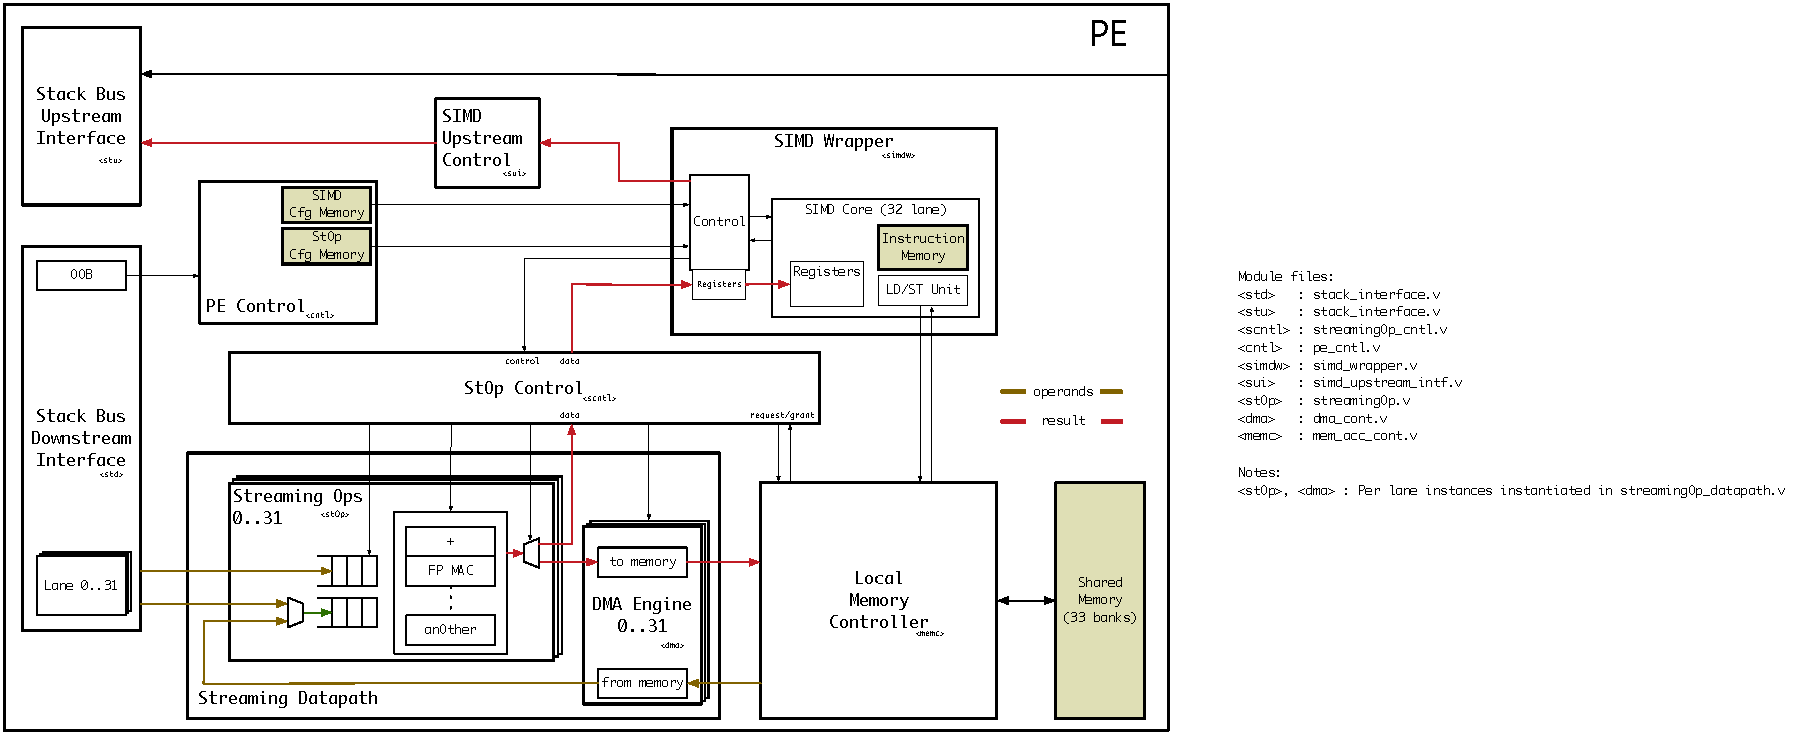
\includegraphics[width=1\linewidth]{PE}}
}
\center\caption{PE block diagram}
\label{fig:PE block diagram}
\end{figure}

\subsection{Configuration}
\label{sec:peConfiguration}

A configuration controller within the PE (PE\_CNTL) takes the OOB packet from the Manager and extracts the stOp and SIMD operation pointers.

The stOp pointer is used to point to a local stOp configuration memory. The memory contains the various configuration data required by the streaming operation controller (stOp\_CNTL). The stOp\_CNTL is not shown.

The stOp\_CNTL configures the:

\begin{outline}
    \1 Operation type
    \1 Number of active execution lanes
    \1 Source of the argument data, which can be downstream data from the manager or from the small local SRAM
    \1 Destination of the result data, which can be the SIMD or the small local SRAM
\end{outline}

The SIMD operation pointer is sent to the SIMD.

\subsection{Streaming Operations}
\label{ssec:stOps}

The streaming Operations (stOp) are designed to operate on data passed from the Manager at or near line-rate. If line-rate cannot be maintained, a flow-control mechanism is employed to slow the data from the Manager.

Once the stOp has processed the data, it passes the result to the SIMD. Note in some cases the result can be placed in local SRAM or sent to both SIMD and SRAM.

It should also be stated that while the stOp is processing the current data, the SIMD may be operating on the result of the previous operation. It is expected the SIMD will have completed the previous operation before the stOp completes the current operation, but again, if necessary a flow control mechanism between SIMD and stOP will be engaged if the SIMD is not ready.

\subsection{SIMD}
\label{ssec:simd}

The SIMD takes the result data and performs the operation starting at the program counter (PC) indicated by the SIMD operation pointer provided by the PE\_CNTL.

The stOp provides the result to the SIMD via a local register. The result is also written, in most cases to the small local SRAM.

The SIMD performs the specified operation on the data provided by the stOp.

In most cases this will be the AN activation function and in the baseline system is the Rectified Linear function (ReLu).

When the SIMD has completed its operation, it passes the result to the SIMD Upstream controller to be returned to the Manager.

\subsection{Result Data}
\label{ssec:result}

The SIMD Upstream Controller (SUI) takes the data and encapsulates it in an Upstream packet. Included in the packet is the tag required by the Return Data processor within the Manager.



